\documentclass[twoside,twocolumn]{article}

\usepackage{blindtext} 
\usepackage{graphicx}
\usepackage[sc]{mathpazo} 
\usepackage[T1]{fontenc} 
\linespread{1.05} 
\usepackage{microtype} 


\usepackage[english]{babel} 


\usepackage[hmarginratio=1:1,top=32mm,columnsep=20pt]{geometry} 
\usepackage[hang, small,labelfont=bf,up,textfont=it,up]{caption} 
\usepackage{booktabs} 


\usepackage{lettrine} 


\usepackage{enumitem} 
\setlist[itemize]{noitemsep} 


\usepackage{abstract} 
\renewcommand{\abstractnamefont}{\normalfont\bfseries} 
\renewcommand{\abstracttextfont}{\normalfont\small\itshape} 


\usepackage{titlesec} 
\renewcommand\thesection{\Roman{section}} % 
\renewcommand\thesubsection{\roman{subsection}} 
\titleformat{\section}[block]{\large\scshape\centering}{\thesection.}{1em}{} 
\titleformat{\subsection}[block]{\large}{\thesubsection.}{1em}{} 


\usepackage{fancyhdr} 
\pagestyle{fancy} 
\fancyhead{} 
\fancyfoot{} 
\fancyhead[C]{Titulo $\bullet$ Junio 2019 $\bullet$ } 
\fancyfoot[RO,LE]{\thepage} 


\usepackage{titling} 


\usepackage{hyperref} 


%----------------------------------------------------------------------------------------
%	TILULOS
%----------------------------------------------------------------------------------------


\setlength{\droptitle}{-4\baselineskip} 

\pretitle{\begin{center}\Huge\bfseries} 
\posttitle{\end{center}} 
\title{Business Intelligence and Business Analytics} 
\author{Franklin Carlos Huichi Contreras, Jose Pastor, Sigfredo, \\
 Sandoval. }
\date{\today} 
\renewcommand{\maketitlehookd}{
\begin{abstract}
\noindent 
asdasdasdasdadasdasdasdasdads asdasdasdasdadasdasdasdasdads asdasdasdasdadasdasdasdasdads asdasdasdasdadasdasdasdasdadsasdasdasdasdadasdasdasdasdads 
asdasdasdasdadasdasdasdasdads asdasdasdasdadasdasdasdasdadsasdasdasdasdadasdasdasdasdadsasdasdasdasdadasdasdasdasdads asdasdasdasdadasdasdasdasdads 
asdasdasdasdadasdasdasdasdads asdasdasdasdadasdasdasdasdads asdasdasdasdadasdasdasdasdads asdasdasdasdadasdasdasdasdads
\end{abstract}
\begin{abstract}
\noindent 
asdasdasdasdadasdasdasdasdads asdasdasdasdadasdasdasdasdads asdasdasdasdadasdasdasdasdads asdasdasdasdadasdasdasdasdadsasdasdasdasdadasdasdasdasdads 
asdasdasdasdadasdasdasdasdads asdasdasdasdadasdasdasdasdadsasdasdasdasdadasdasdasdasdadsasdasdasdasdadasdasdasdasdads asdasdasdasdadasdasdasdasdads 
asdasdasdasdadasdasdasdasdads asdasdasdasdadasdasdasdasdads asdasdasdasdadasdasdasdasdads asdasdasdasdadasdasdasdasdads

\end{abstract}
}

%----------------------------------------------------------------------------------------

\begin{document}

% Print the title
\maketitle

%----------------------------------------------------------------------------------------
%	INTRODUCCION
%----------------------------------------------------------------------------------------

\section{Introduccion}
\lettrine[nindent=0em,lines=3]{A}sdasdasdasdasdasdasdadasdasdasdasdads asdasdasdasdadasdasdasdasdads asdasdasdasdadasdasdasdasdads asdasdasdasdadasdasdasdasdadsasdasdasdasdadasdasdasdasdads asdasdasdasdadasdasdasdasdads asdasdasdasdadasdasdasdasdads asdasdasdasdadasdasdasdasdads asdasdasdasdadasdasdasdasdads asdasdasdasdadasdasdasdasdads asdasdasdasdadasdasdasdasdads asdasdasdasdadasdasdasdasdads asdasdasdasdadasdasdasdasdads asdasdasdasdadasdasdasdasdads asdasdasdasdadasdasdasdasdads asdasdasdasdadasdasdasdasdads asdasdasdasdadasdasdasdasdads asdasdasdasdadasdasdasdasdads


%----------------------------------------------------------------------------------------
%	Objetivos
%----------------------------------------------------------------------------------------


\section{Marco teorico}

\begin{itemize}
\item Inteligencia de Negocios (BI): \\ 
La inteligencia de negocios es el proceso de recopilar, almacenar y analizar datos de operaciones empresariales. La inteligencia de negocios ofrece metricas integrales de negocio,
en tiempo real con el fin de poder mejorar la toma de decisiones. Con una mejor inteligencia de negocio podemos crear valores de referencia de rendimiento, detectar tendencia del mercado,
aumentar el cumplimiento y mejorar en todos los aspectos de la empresa.
\begin{center}
	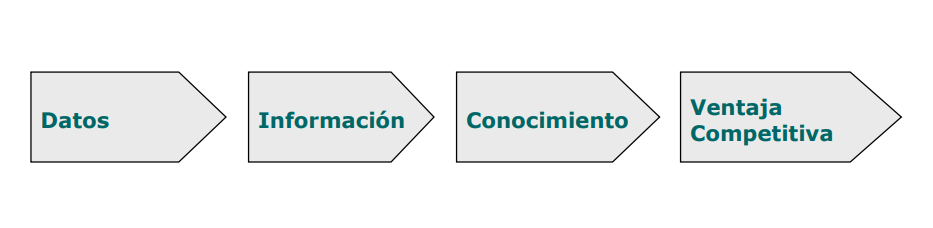
\includegraphics[width=7cm]{./Imagenes/bi} 
\end{center}

\item Analisis de Negocio (BA): \\ 
El análisis de negocio es el conjunto de métodos y técnicas utilizadas para trabajar como enlace entre los stakeholders con el fin de comprender la estructura, políticas y operaciones de una organización y recomendar soluciones que permitan alcanzar sus objetivos. El análisis de negocio implica la comprensión de cómo funcionan las organizaciones para llevar a cabo sus propósitos y la definición de las capacidades que requiere para proporcionar productos y servicios a los grupos de interés externos.

\end{itemize}



%----------------------------------------------------------------------------------------
%	DESARROLLO
%----------------------------------------------------------------------------------------

\section{Desarrollo}

\subsection{¿Que no es Business Intelligence?}
Comencemos con los que no es BI. BI no es:
Un solo producto. Aunque muchos productos excelentes pueden ayudarlo a implementar BI, BI no es un producto que se pueda comprar e instalar para resolver todos sus problemas "desde el primer momento". BI tampoco es una tecnologia, aunque las herramientas y tecnologías de DW, como las herramientas ETL de bases de datos relacionales, las herramientas de interfaz de usuario de BI y los servidores, se usan típicamente para admitir aplicaciones de BI. BI no es solamente una tecnologia.

\subsection{Si eso es lo que BI no es, ¿Entonces qué es?}
BI combina productos, tecnología y métodos para organizar la información clave que la gerencia necesita para mejorar las ganancias y el rendimiento. En términos más generales, pensamos en bi como información comercial y análisis de negocios dentro del contexto de procesos comerciales clave que conducen a decisiones y acciones, Que resultan en un mejor desempeño comercial, en particular BI significa apalancar los activos de información dentro de los procesos comerciales clave para lograr un mejor rendimiento comercial. Incluye información y análisis de negocios que son:

\begin{itemize}	
	\item Utilizado dentro de un contexto de procesos comerciales clave.
	\item Apoyar decisiones y acciones.
	\item Conducir a un mejor rendimiento empresarial.

\end{itemize} 

\subsection{¿Que es Business Analytics}

Business analytics es un campo que impulsa cambios prácticos basados en datos en una empresa. Es una aplicación práctica de análisis estadístico que se centra en proporcionar recomendaciones viables. Los analistas en este campo se centran en cómo aplicar los conocimientos que derivan de los datos. Su objetivo es sacar conclusiones concretas sobre un negocio respondiendo preguntas específicas sobre por qué sucedieron las cosas, qué sucederá y qué se debe hacer.
 
El análisis cuando se aplica a los datos, crea información. en su forma más amplia, abarca una amplia gama de disciplinas, incluidas la inteligencia empresarial, las estadísticas, la gestión de datos y la ciencia de datos. Por ejemplo, el análisis avanzado y el aprendizaje automático es un subconjunto de análisis que se enfoca en extraer una mayor comprensión a través de técnicas matemáticas. A menudo trata de entender por qué suceden las cosas y predecir lo que sucederá en lugar de simplemente resumir lo que ya sucedió. una vez creado, se necesita actuar sobre la información para crear valor. donde el análisis crea información, BA se preocupa por tomar esa información y usarla para crear valor.

\begin{center}
	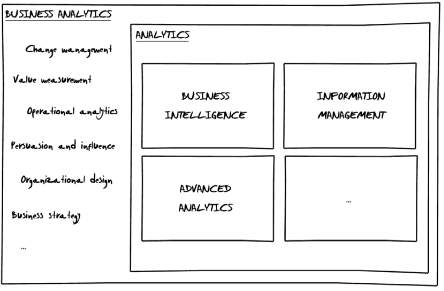
\includegraphics[width=7cm]{./Imagenes/ba} 
\end{center}

\subsection{¿En que se diferencian Business Intelligence con Business Analytics?}
\begin{itemize}	
	\item La diferencia principal en ambas ideas es que el Business Inteligence se enfoca en los datos que manejamos los datos ya recopilados la cual la podemos convertir en informacion y usarla para analizarlas y entender el pasado del negocio. Por otro lado el Business Analytics nos permitira centrarnos en el presente para crear una vision clara del futuro y predecir (mediante modelos predectivos) para adelantarnos al futuro.
	\item La  diferencia entre los dos radica en comprender el valor de la percepción y convencer a una organización para que cambie la forma en que hace negocios.
\end{itemize} 





\subsection{¿En que se asemejan Business Intelligence con Business Analytics?}
Business Intelligence y Business Analytics se basan en la recopilacion de datos de una empresa para convertirlos en informacion y usarla para los analisis, asimismo mostrar graficos estadisticas para el mejor aprovechamiento de la informacion y asi tomar las mejores decisiones de negocios.



%----------------------------------------------------------------------------------------
%	CONCLUSIONES
%----------------------------------------------------------------------------------------

%----------------ESTO LO HIZO EL OTRO TEAMMMMMM :v :V -----------------------------------------------------------------------
%----------------ESTO LO HIZO EL OTRO TEAMMMMMM :v :V -----------------------------------------------------------------------
%----------------ESTO LO HIZO EL OTRO TEAMMMMMM :v :V -----------------------------------------------------------------------
%----------------ESTO LO HIZO EL OTRO TEAMMMMMM :v :V -----------------------------------------------------------------------
%----------------HAY QUE CAMBIARLO -----------------------------------------------------------------------
%----------------HAY QUE CAMBIARLO -----------------------------------------------------------------------
%----------------HAY QUE CAMBIARLO -----------------------------------------------------------------------
%----------------HAY QUE CAMBIARLO -----------------------------------------------------------------------


\section{Conclusiones}
\begin{itemize}	
	\item CONCLUYO QUE ESTA ES UNA CONCLUSION

\end{itemize} 



%----------------------------------------------------------------------------------------
%	BIBLIOGRAFIA
%----------------------------------------------------------------------------------------


\begin{thebibliography}{99} 

\bibitem[Silvia Chavez y Carmen Contreras, 2018]{}
\newblock Implementación de Business Intelligence, para el proceso de toma de decisiones del área de ventas.

\bibitem[Hans Peter Luhn 1958]{}
\newblock A Business Intelligence System

\bibitem[Alex Rayón, 2015]{Universidad de Deusto}
Conceptos básicos del Business Intelligence.

\bibitem[Jordi Conesa y Josep Curto, 2010]{}
\newblock Introduccion al Business Intelligence

\bibitem[Margaret Rouse, 2019]{}
\newblock Análisis de negocios (BA)

\bibitem[Noodle Editorial Staff, 2018]{}
\newblock Business analytics career paths

\bibitem[Josep Lluis Cano, 2007]{}
\newblock Business Intelligence: competir con información


\bibitem[Curto J., 2010]{} 
\newblock Introducción al Business Intelligence. Editorial UOC.

\bibitem[Kimball R. and Ross M., 2002]{} 
\newblock  The Data Warehouse Toolkit: The Complete Guide to Dimensional Modeling. Wiley

\bibitem[Carolina A., 2017]{} 
\newblock  Análisis de Negocio (Business Analysis, BA)
 
\end{thebibliography}


%----------------------------------------------------------------------------------------


\end{document}
